% requires LaTeX (LaTeX2e)
\documentclass[12pt]{article}

% ****************** BASIC FORMATTING ************************

\setlength{\textheight}{9.0in}
\setlength{\textwidth}{6.5in}
\setlength{\topmargin}{0in}
\setlength{\headheight}{0in}
\setlength{\headsep}{0in}
%\setlength{\footskip}{0in}
\setlength{\oddsidemargin}{0in}
\setlength{\evensidemargin}{0in}
\setlength{\marginparsep}{0in}
\setlength{\marginparwidth}{0in}

% ****************** BIBLIOGRAPHY ************************

%\usepackage{AMS}
\bibliographystyle{AMS}

% ****************** GRAPHICS ************************

\usepackage[final]{graphicx} % works with latex, pdflatex--leave off extensions

% ****************** OTHER PACKAGES ************************

% HYPERREF:  This package creates hyperlinks to equations, sections, 
% references, etc.  It works with either LaTeX or pdflatex
% and the resulting links work with acrobat, xpdf, and xdvi
% PUT THIS EARLY--IT POLLUTES THE NAMESPACE WITH THINGS LIKE \v
%\usepackage{hyperref}

\usepackage{amssymb, amsmath, amsfonts}

% ****************** MORE FORMATTING ************************

%\setlength{\parindent}{0pt}
\setlength{\parskip}{12pt plus6pt minus3pt}
\setlength{\jot}{6pt} % extra space between equations in \eqnarray or \align

% commands to number equations by section, e.g., (2.3):
\renewcommand{\theequation}{\thesection.\arabic{equation}}
% NOTE:  you must also reset the equation counter "equation" at each section:
%\section{Title of Section}
%\setcounter{equation}{0}

% macros for narrower captions:
% \mycaption{text}
% \Mycaption{width}{text}
\newcommand{\mycaption}[1]{\Mycaption{5.5in}{#1}}
\newcommand{\Mycaption}[2]{\parbox[t]{#1}{\caption{#2}}}

% ****************** SYMBOLS ************************

\usepackage{amsfonts}
\newcommand{\R}{\mathbb{R}}
\newcommand{\C}{\mathbb{C}}
\newcommand{\dx}{\Delta x}
\newcommand{\dt}{\Delta t}
\newcommand{\half}{\frac12}
\newcommand{\ubar}{\bar{u}}
\newcommand{\vbar}{\bar{v}}
\newcommand{\href}{\bar{h}}
\newcommand{\cbar}{\bar{c}}
\newcommand{\etaref}{\bar{\eta}}
\newcommand{\kbar}{\bar{k}}
\newcommand{\omegabar}{\bar{\omega}}
\renewcommand{\u}{\mathbf{u}}
\renewcommand{\v}{\mathbf{v}}
\newcommand{\w}{\mathbf{w}}
\renewcommand{\a}{\mathbf{a}}
\newcommand{\A}{\mathbf{A}}
\newcommand{\opA}{\mathcal{A}}
\newcommand{\opB}{\mathcal{B}}
\newcommand{\opC}{\mathcal{C}}
\newcommand{\opL}{\mathcal{L}}
\renewcommand{\b}{\mathbf{b}}
\renewcommand{\c}{\mathbf{c}}
\newcommand{\f}{\mathbf{f}}
\newcommand{\F}{\mathbf{F}}
\newcommand{\g}{\mathbf{g}}
\newcommand{\h}{\mathbf{h}}
\newcommand{\Fr}{\mbox{Fr}}
\newcommand{\cross}{\times}
\newcommand{\del}{\nabla}
\newcommand{\Span}{\mbox{span}\,}
\renewcommand{\Re}{\mbox{Re}\,}
\renewcommand{\Im}{\mbox{Im}\,}
\newcommand{\laplacian}[1]{\del^2#1}
%\newcommand{\fluxdiv}[2]{\mathcal{F}\left(#1,#2\right)}
\newcommand{\fluxdiv}[2]{\del\cdot\left(#1\del#2\right)}
\newcommand{\jacobian}[2]{\mathcal{J}\left(#1,#2\right)}

% absolute value, norm, condition number, and inner product:
%     \abs{stuff}
%     \norm{stuff}  or \norm[type]{stuff}   ex:  \norm[\infty]{x}
%     \cond{stuff}  or \cond[type]{stuff}   ex:  \cond[2]{x}
%     \ip{arg}{arg} or \ip[type]{arg}{arg}  ex:  ex:  \ip[A]{f}{g}
\newcommand{\abs}[1]{\left|{#1}\right|}
\newcommand{\norm}[2][{}]{\ensuremath{\left\|{#2}\right\|_{#1}}}
\newcommand{\cond}[2][{}]{\ensuremath{\text{cond}\!\left({#2}\right)}_{#1}}
\newcommand{\ip}[3][{}]{\ensuremath{\left\langle{#2},{#3}\right\rangle_{#1}}}


% ****************** OTHER DEFINITIONS ************************

\newcommand{\units}[1]{\,\mbox{#1}}

% ****************** FRONT MATTER ************************

\title{Semi-Implicit Discretization \\
of the Shallow-Water Equations}

\author{Scott R. Fulton
%\\[12pt]
%\emph{Department of Mathematics and Computer Science}\\
%\emph{Clarkson University, Potsdam, NY 13699--5815}
}

\date{15 June 2007}
%\date{Revised \today}

% ****************** START OF DOCUMENT ************************

\begin{document}
\maketitle

% ****************** ABSTRACT ************************

\begin{abstract}

%\noindent

The shallow-water equations admit both fast (gravity-inertia) and slow
(Rossby) modes.  In most situations of meteorological and oceanographic
interest the fast modes contain little energy.  Therefore, semi-implicit time
discretization has the potential to increase the time step beyond the explicit
CFL limit without compromising accuracy.  These notes analyze the linearized
shallow-water equations to identify which terms should be treated implicitly
and explicitly.  Based on this analysis, appropriate splittings are developed
for various forms of the nonlinear shallow-water equations.  Finally, the
properties of various discretizations are surveyed to motivate the choice of a
good semi-implicit scheme.

\end{abstract}

\thispagestyle{empty}



% ****************** TEXT ************************

\pagebreak[4]
\section{Introduction}
\setcounter{equation}{0}

\newcommand{\vecv}{\mathbf{v}}
\newcommand{\vecV}{\mathbf{V}}
\newcommand{\veck}{\mathbf{k}}
\newcommand{\Fmom}{\mathbf{F}}
\newcommand{\Fmass}{F_h}
\newcommand{\Feta}{F_{\eta}}
\newcommand{\Fdelta}{F_{\delta}}
\newcommand{\solvec}{\psi}
The shallow-water equations include advective, Coriolis, and pressure gradient
terms, and thus serve as a prototype for general primitive-equation models.
We can write the momentum and mass continuity equations in the form
\begin{align}
  \frac{\partial \vecv}{\partial t} + \vecv\cdot\del\vecv 
    + f\veck\cross\vecv + g\del h &= \Fmom, 
\label{SW:momentum}
\\
  \frac{\partial h}{\partial t} + \del\cdot(h\vecv) &= \Fmass,
\label{SW:continuity}
\end{align}
where $\vecv$ is the (horizontal) vector velocity, $h$ is the free surface
height, $f$ is the Coriolis parameter, $g$ is the gravitational constant,
$\veck$ is the vertical unit vector, and the operator $\del$ is restricted to
the horizontal.  The source terms $\Fmom$ and $\Fmass$ for momentum and mass
are regarded as known functions of $t$ (and possibly of $\vecv$ and $h$).
Other forms of these equations will also be considered below.

It is well-known that the shallow-water equations admit both fast
(gravity-inertia) and slow (Rossby) modes.  In most situations of
meteorological and oceanographic interest, only the slow modes are of
interest, and the fast modes contain little energy.  Therefore, a natural 
(and common) solution procedure is to split the terms in the equations into
two groups, namely, those related to the fast and slow modes, and treat the
former implicitly and the latter explicitly.  Such a \emph{splitting} can be
written generically in the form
\begin{equation}
  \solvec'(t) = \opA(\solvec(t)) + \opB(\solvec(t)) ,
\label{ODE}
\end{equation}
where the vector $\solvec$ represents the solution at time~$t$ and the
operators $\opA$ and $\opB$ represent the terms to be treated implicitly and
explicitly, respectively.  For example, if the space dependence is left
continuous, we can set $\solvec = [u,v,h]^T$, where $u$ and $v$ are components
of the vector velocity.  Likewise, if the equations are discretized in space
(e.g., by a finite-difference or spectral method), we can set $\solvec =
[\u^T,\v^T,\h^T]^T$, where the components are (mathematical) vectors (e.g.,
collections of gridpoint values or spectral coefficients) representing $u$,
$v$, and $h$ at time~$t$.  Similar interpretations of $\solvec$ are possible
for other forms of the shallow-water equations (see below).

We consider discretizations of \eqref{ODE} which replace the solution
$\solvec(t)$ with an approximation $\solvec^n\approx \solvec(t_n)$ at times
$t_n=n\dt$ for $n=0,1,\dots$.  A \emph{semi-implicit} discretization treats
$\opA(\solvec)$ implicitly and $\opB(\solvec)$ explicitly, i.e., it reduces to
an explicit method if $\opA(\solvec)\equiv0$ and to an implicit method if
$\opB(\solvec)\equiv0$.  The simplest such scheme combines the backward
(implicit Euler) and forward (explicit Euler) schemes to give the
discretization
\begin{equation}
  \frac{\solvec^{n+1}-\solvec^{n}}{\dt} = \opA(\solvec^{n+1}) + \opB(\solvec^{n}) .
\label{BACK-FOR}
\end{equation}
The scheme most often used in meteorological models (e.g., 
\cite{Kwizak_Robert71, Cote_Beland_Staniforth83, Simmons_Hoskins_Burridge78,
Staniforth_Daley79})
combines the trapezoidal (implicit) and leapfrog (explicit) schemes, yielding
the discretization 
\begin{equation}
  \frac{\solvec^{n+1}-\solvec^{n-1}}{2\dt} =
\frac{\opA(\solvec^{n-1})+\opA(\solvec^{n+1})}{2} 
    + \opB(\solvec^{n}) .
\label{TRAP-LFG}
\end{equation}
As we will see in section~\ref{sec:analysis} below, more general
combinations of linear multistep methods are possible.\footnote{It is also
possible to formulate semi-implicit schemes based on Runge-Kutta methods.
For example, combining the backward and fourth-order Runge-Kutta methods
generates a scheme which works well for problems of the advection-diffusion
type \cite{Fulton93}.  However, an extensive search \cite{Kang94} suggests
that no such schemes exist with stability properties appropriate for
oscillatory problems like the shallow-water equations; see also
section~\ref{sec:abstab}.} Any such scheme results in an implicit problem of
the form
\begin{equation}
  \solvec^{n+1}-\tau\opA(\solvec^{n+1}) = \opC^{n},
\label{eq:implicit}
\end{equation}
where $\tau$ is a multiple of the time step ($\tau=\dt$ for the two schemes
above) and $\opC^{n}$ is a combination of values of $\opA(\solvec)$ and
$\opB(\solvec)$ which are known at time~$t_n$.  The execution of one time step
thus consists of first computing $\opC^{n}$ and then solving
\eqref{eq:implicit}---with appropriate boundary conditions---for
$\solvec^{n+1}$.

Formulating a good semi-implicit scheme for the shallow-water equations thus
involves two choices:
\begin{itemize} 
\setlength{\itemsep}{1pt} \setlength{\parsep}{0pt}
\setlength{\topsep}{0pt} \setlength{\partopsep}{0pt}
\item
\emph{Splitting}:  
which terms should be treated implicitly and explictly?
\item
\emph{Discretization}:  
which implicit and explicit disretizations should be used?
\end{itemize} 
The purpose of these notes is to answer these questions.  First, the choice of
splitting involves identifying the terms responsible for the fast modes; this
we do in section~\ref{sec:SWanalysis} by analyzing the linearized
shallow-water equations.  The choice of splitting also affects the complexity
of the resulting implicit problem \eqref{eq:implicit}; the forms this takes
for various forms of the shallow-water model are derived in
section~\ref{sec:splitting}.  Section~\ref{sec:analysis} defines general
semi-implicit schemes based on linear multistep methods and summarizes
conditions for their consistency and convergence.  Absolute stability is
defined and analyzed in section~\ref{sec:abstab}, and a particularly promising
semi-implicit scheme is identified.  Section~\ref{sec:conclusions} summaries
the conclusions.

\pagebreak[4]
\section{Linear analysis\label{sec:SWanalysis}}
\setcounter{equation}{0}

To justify a proper splitting of terms for semi-implicit time differencing, we
use the following linear analysis.\footnote{A linear analysis based on the
vorticity/divergence form yields the same conclusions.}   Assuming that $f$ is
constant and the forcing vanishes, and using Cartesian coordinates with
velocity components $u$ and $v$ in the $x$ and $y$ directions, we can
linearize \eqref{SW:momentum}--\eqref{SW:continuity} about a constant basic
state with velocity $(\ubar,\vbar)$ and height $\href>0$ to obtain
\begin{align}
  u_t + \ubar u_x + \vbar u_y - fv + gh_x &= 0 , 
\label{SW:u:linear}\\
  v_t + \ubar v_x + \vbar v_y + fu + gh_y &= 0 , 
\label{SW:v:linear}\\
  h_t + \ubar h_x + \vbar h_y + \href(u_x + v_y) &= 0 .
\label{SW:h:linear}
\end{align}
Here, $h$ now denotes the \emph{deviation} of the free surface height from the
reference height $\href$, and subscripts denote partial derivatives.  Scaling
$h$ by $g/c$, where $c:=\left(g\href\right)^{1/2}$ is the phase speed of a
pure gravity wave, we can write \eqref{SW:u:linear}--\eqref{SW:h:linear} in the
symmetrized matrix form
\begin{equation}
  \dfrac{\partial\solvec}{\partial t} = \opL\solvec ,
\end{equation}
where $\solvec = \left[ u, v, gh/c \right]^T$ and
\begin{equation}
  \opL = \begin{bmatrix}
       -\ubar\partial_x - \vbar\partial_y & f & -c\partial_x \\
      -f & -\ubar\partial_x - \vbar\partial_y & -c\partial_y \\
      -c\partial_x & -c\partial_y & -\ubar\partial_x - \vbar\partial_y \\
      \end{bmatrix} .
\end{equation}
Assuming wave-form solutions, i.e., $\solvec(x,y,t) = \hat\solvec(t) e^{i(kx+ly)}$, 
leads to
\begin{equation}
  \dfrac{d\hat\solvec}{dt} = L\hat\solvec,
\label{SW:matrix}
\end{equation}
where
\begin{equation}
  L = \begin{bmatrix}
       -i\omegabar & f & -ikc \\
      -f & -i\omegabar & -ilc \\
      -ikc & -ilc & -i\omegabar \\
      \end{bmatrix}
\end{equation}
with $\omegabar := k\ubar + l\vbar$ (which we assume is nonnegative).
Since $L$ is skew-Hermitian, its eigenvalues are pure imaginary.
Writing this eigenvalue problem in the form
$L\Psi_j = -i\omega_j\Psi_j$ for $j=1$, $2$, $3$ (with $\omega_j$ real)
allows us to express the general solution for $\solvec$ as a linear combination 
of solutions of the form 
\begin{equation}
  \solvec(x,y,t) = \Psi_j e^{i(kx+ly-\omega_j t)} .
\end{equation}
Direct calculation yields the following eigenvalues and eigenvectors:
\begin{alignat}{3}
&\mbox{Slow (geostrophic) modes:} & \omega_1 &= \omegabar, & \qquad
   \displaystyle\Psi_1 &= \frac{1}{\nu}\begin{bmatrix}
            -ilc \\ ikc \\ f \end{bmatrix} ,
\\[24pt]
&\mbox{Fast (gravity-inertia) modes:}\quad & \omega_{2,3} &= \omegabar\pm\nu, &
   \displaystyle\Psi_{2,3} &= \frac{1}{\nu\kbar\sqrt{2}}\begin{bmatrix}
            \pm\nu k + ilf \\ \pm\nu l - ikf \\ c\kbar^2 \end{bmatrix} ,
\end{alignat}
where $\nu := (f^2 + \omega_g^2)^{1/2}$, $\omega_g=\kbar c$, and $\kbar :=
(k^2 + l^2)^{1/2}$.  Since $L$ is skew-Hermitian, the eigenvectors $\Psi_j$
are orthogonal in the standard inner product $\ip{\Psi}{\Phi} := \Psi^*\Phi$
(where the asterisk denotes the conjugate transpose); they have been
scaled so that they have unit norm in the corresponding norm
$\norm{\Psi}:=\sqrt{\ip{\Psi}{\Psi}}$.

To determine an appropriate splitting of terms for semi-implicit time
differencing, we write \eqref{SW:matrix} in the form
\begin{equation}
  \dfrac{d\hat\solvec}{dt} = A\hat\solvec + B\hat\solvec + C\hat\solvec,
\label{SW:matrix-split}
\end{equation}
where
\begin{equation}
  A = \begin{bmatrix}
       0 & 0 & -ikc \\
      0 & 0 & -ilc \\
      -ikc & -ilc & 0 \\
      \end{bmatrix},
\quad
  B = \begin{bmatrix}
       -i\omegabar & 0 & 0 \\
      0 & -i\omegabar & 0 \\
      0 & 0 & -i\omegabar \\
      \end{bmatrix},
\quad
  C = \begin{bmatrix}
       \hfill 0 & f & 0 \\
      -f & 0 & 0 \\
      \hfill 0 & 0 & 0 \\
      \end{bmatrix} .
\end{equation}
The matrix $A$ corresponds to the height-gradient term $g\del h$ in the
momentum equation and the divergence term $\href\del\cdot\vecv$ in the
continuity equation, which we identify as the \emph{gravity-wave terms} as
explained below; the matrices $B$ and $C$ correspond to the advective and and
Coriolis terms, respectively.  The corresponding spectral radii
$\rho(A)=\omega_g$, $\rho(B)=\omegabar$, and $\rho(C)=f$ typically satisfy
\begin{equation}
\omega_g\gg\omegabar\gg f ,
\end{equation}
corresponding to a separation of time scales.  In particular, the ratio
$\rho(B)/\rho(A) = \omegabar/\omega_g = \ubar/c$ is the Froude number, which
is typically much smaller than one.  For example, using the values 
$c\sim 300\units{ms$^{-1}$}$,
$\ubar\sim 30\units{ms$^{-1}$}$,
$f\sim 10^{-4}\units{s$^{-1}$}$, and
$\kbar\sim 2\pi/(200\units{km})$
leads to $\omega_g/\omegabar \sim 10$ and $\omegabar/f\sim 10$. 
Thus, we can think of the terms $A$, $B$, and $C$ in \eqref{SW:matrix-split}
as the ``fast'', ``slower'', and ``slowest'' terms, respectively.

More precisely, we can quantify which of terms $A$, $B$, and $C$ are important
for which types of motion by computing the size of each term applied to each
of the (normalized) modes $\Psi_j$ ($j=1$, $2$, $3$).  For the slow
(geostrophic) modes ($j=1$) we obtain
\begin{equation}
  \norm{A\Psi_1} = \frac{f\omega_g}{\nu}\approx f,
\qquad
  \norm{B\Psi_1} = \omegabar,
\qquad
  \norm{C\Psi_1} = \frac{f\omega_g}{\nu}\approx f,
\label{SW:sizes:slowmodes}
\end{equation}
where we have used $f\ll\omega_g$ and thus $\omega_g\approx\nu$.
Similarly, for the fast (gravity-inertia) modes ($j=2$, $3$) we obtain
\begin{equation}
  \norm{A\Psi_{2,3}} = \frac{\omega_g}{\nu}
                       \left(\frac{\omega_g^2 + \nu^2}{2}\right)^{1/2}
                     \approx \omega_g,
\quad
  \norm{B\Psi_{2,3}} = \omegabar,
\quad
  \norm{C\Psi_{2,3}} = \frac{f}{\nu}
                       \left(\frac{f^2 + \nu^2}{2}\right)^{1/2}
                     \approx \frac{f}{\sqrt{2}} .
\label{SW:sizes:fastmodes}
\end{equation}
Using the scales assumed above we thus find that the Coriolis terms ($C$) have
(approximate) size $f$ and the advection terms ($B$) have size $10f$ for both
the slow and fast modes, while the gravity-wave terms ($A$) have (approximate) 
size $f$ for the slow modes but $100f$ for the fast modes.  Thus, the terms we
have identified as the ``gravity-wave'' terms indeed are most important for
the fastest components of the solution.  It will be reasonable to treat these
terms implicitly if and only if fast modes contain little energy; in this
situation the advective terms can be treated explicitly, since
they are largest and their time scale is an order of magnitude slower.

One question remains:  should we treat the Coriolis terms implicitly or
explicitly?  Arguments can be made for both approaches.  
Reasons for treating the Coriolis terms explicitly include:
\begin{itemize}
\setlength{\itemsep}{1pt} \setlength{\parsep}{0pt}
\setlength{\topsep}{0pt} \setlength{\partopsep}{0pt}
\item The time scale is slower than for advection, so an implicit method 
is not needed for stability.
\item The resulting implicit system will be simpler.
\end{itemize}
Reasons for treating the Coriolis terms implicitly include:
\begin{itemize}
\setlength{\itemsep}{1pt} \setlength{\parsep}{0pt}
\setlength{\topsep}{0pt} \setlength{\partopsep}{0pt}
\item Implicit methods generally have smaller truncation error than explicit
methods (of the same order), so the accuracy may be higher.
\item Treating the Coriolis and height gradient terms with the same method may
give a better representation of geostrophic balance. 
\item The operators $A+C$ and  $B$ of the associated splitting commute and
thus are orthogonally diagonalizable, so the stability analysis of
section~\ref{sec:abstab} applies directly (to the linear problem), giving some
confidence that methods which the analysis identifies as good will in fact
work properly.  
\end{itemize}
In the next section we detail both of these approaches for the nonlinear
shallow-water equations in various forms.

\pagebreak[4]
\section{Splitting the nonlinear shallow-water
equations\label{sec:splitting}}
\setcounter{equation}{0}

We now seek appropriate splittings for the nonlinear shallow-water equations
based on the above analysis.  To treat the gravity-wave terms implicitly, we
specify a positive reference height $\href$ and set $h=\href+h'$; while
$\href$ must be constant in time it may vary in space (we also consider the
simplifications possible when $\href$ is is constant in space).  In the
sections which follow we develop splittings for the equations in momentum form
and vorticity/divergence form; for each we show how to treat the Coriolis
terms either explicitly or implicitly.

\pagebreak[3]
\subsection{Momentum form}

In the momentum form \eqref{SW:momentum}--\eqref{SW:continuity} of the
shallow-water equations the predictive variables are $\vecv$ and $h$.
While the momentum equation is normally written in the advective form
\eqref{SW:momentum}, in some models (e.g., \cite{Fulton_Schubert87b}) it 
is written in the equivalent rotational form
\begin{equation}
  \frac{\partial \vecv}{\partial t} + (f+\zeta)\veck\cross\vecv 
   + \del(gh+K) = \Fmom, 
\label{SW:rotational}
\end{equation}
where $\zeta = \veck\cdot\del\cross\vecv$ is the relative vorticity and
$K=\frac12\vecv\cdot\vecv$ is the specific kinetic energy.  Since only linear
terms will be treated implicitly and these are identical in both the advective
and rotational forms, both forms of the momentum equation will lead to the
same semi-implicit discretizations.  Therefore, we consider only the momentum
form here.

\pagebreak[2]
\subsubsection{Coriolis terms treated explicitly}

Substituting $h=\href+h'$ into \eqref{SW:momentum}--\eqref{SW:continuity} and
moving the terms to be treated explicitly to the right-hand side yields
\begin{alignat}{2}
  &\frac{\partial \vecv}{\partial t} + g\del h
    &&= \Fmom - \vecv\cdot\del\vecv - f\veck\cross\vecv ,
\label{SW:momentum:split}
\\
  &\frac{\partial h}{\partial t} + \del\cdot(\href\vecv)
    &&= \Fmass - \del\cdot(h'\vecv) .
\label{SW:continuity:split}
\end{alignat}
Comparing \eqref{SW:momentum:split}--\eqref{SW:continuity:split} with
\eqref{ODE}, we see that $\opB$ represents all terms on the right, while
$-\opA$ represents the terms (other than the time derivatives) on the left.
Therefore, for any semi-implicit scheme the implicit problem
\eqref{eq:implicit} corresponding to
\eqref{SW:momentum:split}--\eqref{SW:continuity:split} takes the form
\begin{alignat}{2}
  &\vecv + \tau g\del h &&= \vecV ,
\label{SW:momentum:imp}
\\
  &h + \tau \del\cdot(\href\vecv) &&= H ,
\label{SW:continuity:imp}
\end{alignat}
where $\vecv$ and $h$ now represent the variables \emph{at the new time level}
(i.e., $\solvec^{n+1}$ with the superscript dropped for simplicity), and
$\vecV$ and $H$ are computed explicitly from values at the old time level
(i.e., $\opC^n$ with the superscript dropped for simplicity).

This system is easily solved by eliminating $\vecv$ to obtain the linear
elliptic problem
\begin{equation}
  h - \tau^2\del\cdot\left(\cbar^2\del h\right) = G ,
\label{SW:implicit}
\end{equation}
where $\cbar=\left(g\href\right)^{1/2}$ and
\begin{equation}
 G := H - \tau \del\cdot\left(\href \vecV\right) .
\end{equation}
If $\href$ is constant in space, then \eqref{SW:implicit}
further reduces to the modified Helmholtz equation
\begin{equation}
  h - \tau^2\cbar^2\del^2 h = G .
\label{SW:Helmholtz}
\end{equation}
Solving \eqref{SW:Helmholtz} straightforward (with any space discretization),
and the slight generalization \eqref{SW:implicit} is not much more
difficult in cases where multigrid methods can be used.  Once $h$ is
obtained by solving \eqref{SW:implicit} or \eqref{SW:Helmholtz},
$\vecv$ can be obtained from \eqref{SW:momentum:imp}.

\pagebreak[2]
\subsubsection{Coriolis terms treated implicitly}

If we treat the Coriolis terms implicitly, then \eqref{SW:momentum:split} is
replaced by
\begin{equation}
  \frac{\partial \vecv}{\partial t} + f\veck\cross\vecv + g\del h
    = \Fmom - \vecv\cdot\del\vecv ,
\label{SW:momentum:fsplit}
\end{equation}
where the terms to be treated explicitly are on the right-hand side.  The 
implicit problem corresponding to \eqref{SW:momentum:fsplit} and
\eqref{SW:continuity:split} is
\begin{alignat}{2}
  &\vecv + \tau f\veck\cross\vecv + \tau g\del h &&= \vecV ,
\label{SW:momentum:fimp}
\\
  &h + \tau \del\cdot(\href\vecv) &&= H ,
\label{SW:continuity:fimp}
\end{alignat}
where $\vecV$ is now different than in \eqref{SW:momentum:imp}.
This system also can be solved by eliminating $\vecv$ as follows.  
Taking the cross product of $\tau f\veck$ with \eqref{SW:momentum:fimp}
and subtracting this from \eqref{SW:momentum:fimp} yields
\begin{equation}
 \vecv = a\left[\left(\vecV - \tau f\veck\cross\vecV\right)
           - \tau g\left(\del h - \tau f\veck\cross\del h\right)\right]
\label{SW:v:fimp}
\end{equation}
where $a = \left(1 + \tau^2 f^2\right)^{-1}$ (usually
$|\tau f|\ll1$ so $a\approx1$).  Substituting this into
\eqref{SW:continuity:fimp} yields
\begin{equation}
   h + \tau^2\jacobian{h}{\tau f\cbar^2} 
     - \tau^2\del\cdot\left(\cbar^2\del h\right) = G ,
\label{SW:implicit:fimp}
\end{equation}
where now $\cbar = \left(ag\href\right)^{1/2}$,
$\jacobian{\alpha}{\beta}=\veck\cdot(\del\alpha\cross\del\beta)$ is the
Jacobian operator, and \begin{equation}
   G = H - \tau \del\cdot\left[a\href
      \left(\vecV - \tau f\veck\cross\vecV\right)\right] .
\label{SW:fimp:defG}
\end{equation}
Since $\cbar$ and $f$ are known and $\cbar>0$, \eqref{SW:implicit:fimp} is a
linear elliptic equation for $h$.  It may also be written in the form
\begin{equation}
   h - \tau^2\b\cdot\del h - \tau^2\cbar^2\laplacian{h} = G 
\label{SW:implicit:fimp:alt}
\end{equation}
where
\begin{equation}
   \b = \del\left(\cbar^2\right) 
      + \tau\veck\cross\del\left(f\cbar^2\right) .
\end{equation}
If $\href$ does not vary too rapidly in space, the first-order term in
\eqref{SW:implicit:fimp} [or \eqref{SW:implicit:fimp:alt}] will be relatively
small so the second-order term will dominate; thus we should be able to solve
this equation for $h$ using standard methods.  The corresponding velocity
$\vecv$ then can be computed from \eqref{SW:v:fimp}.
Note that if $f$ is constant (i.e., an $f$-plane) and $\href$ is constant,
then $\b=0$ and \eqref{SW:implicit:fimp:alt} reduces to the modified 
Helmholtz equation \eqref{SW:Helmholtz}, but this time with $G$ given by 
\eqref{SW:fimp:defG}.

\pagebreak[3]
\subsection{Vorticity/divergence form}

The momentum form \eqref{SW:momentum}--\eqref{SW:continuity} treated above has
the disadvantage that the components of the velocity $\vecv$ are not true
scalars (their values depend on the coordinate system chosen).  Thus, some
authors advocate using vorticity and divergence instead
(e.g.,~\cite{Heikes_Randall95a}).  To do so, we take the dot product of
$\veck$ with the curl of the momentum equation in the form
\eqref{SW:rotational} to obtain the vorticity equation 
\begin{equation}
   \frac{\partial \eta}{\partial t} + \del\cdot(\eta\vecv) =
      \Feta := \veck\cdot\del\cross\Fmom .
\label{SW:vorticity}
\end{equation}
where $\eta:=f+\zeta$ is the absolute vorticity.  Likewise, taking the
divergence of \eqref{SW:rotational} gives the divergence equation
\begin{equation}
   \frac{\partial \delta}{\partial t} - \veck\cdot\del\cross(\eta\vecv) 
      + \del^2 \left(gh + K\right) = \Fdelta := \del\cdot\Fmom ,
\label{SW:divergence}
\end{equation}
where $\delta = \del\cdot\vecv$ is the divergence.  Combining these equations
with \eqref{SW:continuity} gives a system for predicting $\eta$ (or $\zeta$),
$\delta$, and $h$.  To close this system we introduce a velocity potential
$\chi$ and streamfunction $\psi$ satisfying 
\begin{equation}
   \vecv = \del\chi + \veck\cross\del\psi .
\label{SW:wind}
\end{equation}
Then the velocity $\vecv$ can be obtained from $\zeta$ and $\delta$ by solving
the Poisson problems
\begin{equation}
   \del^2\psi = \zeta, \qquad \del^2\chi = \delta 
\label{SW:Poisson}
\end{equation}
(with appropriate boundary conditions) and using \eqref{SW:wind}.  

\pagebreak[2]
\subsubsection{Coriolis terms treated explicitly}

Substituting $h=\href+h'$ into \eqref{SW:vorticity}--\eqref{SW:divergence} and
moving the terms to be treated explicitly to the right-hand side yields
\begin{equation}
   \frac{\partial \zeta}{\partial t} = \Feta - \del\cdot(\eta\vecv)
\label{SW:vorticity:split}
\end{equation}
and
\begin{equation}
   \frac{\partial \delta}{\partial t} + g\del^2 h = 
      \Fdelta + \veck\cdot\del\cross(\eta\vecv) - \del^2 K.
\label{SW:divergence:split}
\end{equation}
Combining these equations with \eqref{SW:continuity:split} and treating the
terms on the left implicitly and those on the right explicitly, the
corresponding implicit problem [cf.~\eqref{eq:implicit}] takes the form
\begin{alignat}{2}
   &\zeta &&= Z,
\label{VD:vorticity:imp}
\\
   &\delta  + \tau g\del^2 h &&= D,
\label{VD:divergence:imp}
\\
  &h + \tau \del\cdot(\href\vecv) &&= H ,
\label{VD:continuity:imp}
\end{alignat}
where $\zeta$, $\delta$, $h$, and $\vecv$ are values at the new time level and
related by \eqref{SW:wind} and \eqref{SW:Poisson}, and $Z$, $D$, and $H$ are
computed explicitly from values at the old time level.  

\newcommand{\chihat}{\hat\chi}

To solve this system, first note that \eqref{VD:vorticity:imp} gives $\zeta$
explicitly, so we can determine $\psi$ by solving \eqref{SW:Poisson}. 
If $\href$ is constant then \eqref{VD:continuity:imp} reduces to
\begin{equation}
  h + \tau \href\delta = H .
\label{VD:continuity:imp:Hconst}
\end{equation}
Eliminating $\delta$ between \eqref{VD:continuity:imp:Hconst} and
\eqref{VD:divergence:imp} yields the Helmholtz problem
\begin{equation}
   h - \tau^2\cbar^2\del^2 h = G ,
\label{VD:Helmholtz:nof}
\end{equation}
[cf.~\eqref{SW:Helmholtz}], where $\cbar = \left(g\href\right)^{1/2}$ and 
\begin{equation}
   G = H - \tau \href D .
\end{equation}
Once \eqref{VD:Helmholtz:nof} is solved for $h$, the corresponding $\delta$
can be obtained from \eqref{VD:continuity:imp:Hconst}, then $\chi$ from
\eqref{SW:Poisson}, and $\vecv$ from \eqref{SW:wind}.  Even if $\href$ is not
constant, we can still eliminate $\delta$ by first introducing 
\begin{equation}
   \chihat := \chi + \tau gh
\label{def:chihat}
\end{equation}
to write \eqref{VD:divergence:imp} as
\begin{equation}
   \laplacian\chihat = D .
\label{eq:chihat}
\end{equation}
Assuming we can solve this (with appropriate boundary conditions) for
$\chihat$, we can then substitute for $\vecv$ in \eqref{VD:continuity:imp}
from \eqref{SW:wind} and eliminate $\chi$ using \eqref{def:chihat} to obtain
the linear elliptic equation
\begin{equation}
   h - \tau^2\del\cdot\left(\cbar^2\del h\right) = G 
\label{VD:nof}
\end{equation}
[cf.~\eqref{SW:implicit}], where
\begin{equation}
   G = H - \tau\del\cdot(\href\del\chihat) + \tau\jacobian{\href}{\psi} .
\end{equation}
Once \eqref{VD:nof} is solved for $h$, we can compute $\chi$ from
\eqref{def:chihat}, $\delta$ from \eqref{SW:Poisson}, and $\vecv$ from
\eqref{SW:wind}.

\pagebreak[2]
\subsubsection{Coriolis terms treated implicitly}

If we treat the Coriolis terms implicitly, then \eqref{SW:vorticity:split} 
and \eqref{SW:divergence:split} are replaced by
\begin{equation}
   \frac{\partial \zeta}{\partial t} + \del\cdot(f\vecv) =
      \Feta - \del\cdot(\zeta\vecv)
\label{SW:vorticity:fsplit}
\end{equation}
and
\begin{equation}
   \frac{\partial \delta}{\partial t} - \veck\cdot\del\cross(f\vecv)
      + g\del^2 h = \Fdelta    + \veck\cdot\del\cross(\zeta\vecv) - \del^2 K.
\label{SW:divergence:fsplit}
\end{equation}
Combining these equations with \eqref{SW:continuity:split} and treating the
terms on the left implicitly and those on the right explicitly, the
corresponding implicit problem [cf.~\eqref{eq:implicit}] takes the form
\begin{alignat}{2}
   &\zeta + \tau\del\cdot(f\vecv) &&= Z,
\label{VD:vorticity:fimp}
\\
   &\delta - \tau\veck\cdot\del\cross(f\vecv) + \tau g\del^2 h &&= D,
\label{VD:divergence:fimp}
\\
  &h + \tau \del\cdot(\href\vecv) &&= H ,
\label{VD:continuity:fimp}
\end{alignat}
where again $\zeta$, $\delta$, $h$, and $\vecv$ are values at the new time
level and related by \eqref{SW:wind} and \eqref{SW:Poisson}, and $Z$, $D$, and
$H$ are computed explicitly from values at the old time level.  

In the case of an $f$-plane (i.e., $f$ is constant) with $\href$ constant
also, \eqref{VD:vorticity:fimp}--\eqref{VD:continuity:fimp} reduce to
\begin{alignat}{2}
   &\zeta + \tau f\delta &&= Z ,
\label{VD:vorticity:fplane}
\\
   &\delta - \tau f\zeta + \tau g\laplacian{h} &&= D ,
\label{VD:divergence:fplane}
\\
   &h + \tau\href\delta &&= H .
\label{VD:continuity:fplane}
\end{alignat}
Eliminating $\zeta$ between \eqref{VD:vorticity:fplane} and
\eqref{VD:divergence:fplane} yields
\begin{equation}
   \delta + \tau ag\laplacian{h} = a(D + \tau fZ)
\label{VD:delta}
\end{equation}
where $a = \left(1 + \tau^2 f^2\right)^{-1}$ as before.  Then
eliminating $\delta$ between \eqref{VD:continuity:fplane} and \eqref{VD:delta}
leads to the modified Helmholtz problem
\begin{equation}
   h - \tau^2\cbar^2\del^2 h = G 
\label{VD:Helmholtz}
\end{equation}
[cf.~\eqref{SW:Helmholtz}], where $\cbar = \left(ag\href\right)^{1/2}$
as before and
\begin{equation}
   G = H - \tau a\href(D + \tau fZ).
\end{equation}
Once \eqref{VD:Helmholtz} is solved for $h$ we can compute $\delta$ from
\eqref{VD:continuity:fplane} and $\zeta$ from \eqref{VD:vorticity:fplane}, 
$\psi$ and $\chi$ from \eqref{SW:Poisson}, and $\vecv$ from \eqref{SW:wind}.

\newcommand{\Chi}{X}
Finally, with no simplifying assumptions on $\href$ and $f$, we can in
principle solve the implicit system
\eqref{VD:vorticity:fimp}--\eqref{VD:continuity:fimp} coupled with
\eqref{SW:wind} and \eqref{SW:Poisson} by essentially converting it to the
momentum form as follows.  The key is to introduce the ``forced velocity''
$\vecV$ computed from $Z$ and $D$ as follows.  First, solve
\begin{equation}
   \del^2\Psi = Z, 
\qquad 
\del^2\Chi = D 
\label{Poisson:forcing}
\end{equation}
(with appropriate boundary conditions) for $\Psi$ and $\Chi$.  Then define
\begin{equation}
   \vecV := \del\Chi + \veck\cross\del\Psi ,
\end{equation}
so that $\veck\cdot\del\cross\vecV = Z$ and $\del\cdot\vecV = D$.
Then the velocity $\vecv$ derived from $\psi$, $\chi$, and $h$ satisfying the
implicit system \eqref{VD:vorticity:fimp}--\eqref{VD:continuity:fimp}
satisfies \eqref{SW:momentum:fimp} and \eqref{SW:continuity:fimp}, so we can
solve \eqref{SW:implicit:fimp} for $h$ and compute $\vecv$ from
\eqref{SW:v:fimp}, as explained for the momentum form above.  From
$\vecv$ we can then compute $\delta=\del\cdot\vecv$ and
$\zeta=\veck\cross\del\vecv$ and obtain $\psi$ and $\chi$ by
solving the Poisson problems \eqref{SW:Poisson}.  

\pagebreak[3]
\subsection{Streamfunction/velocity potential form}

While the vorticity/divergence form considered above predicts vorticity and
divergence, it still explicitly involves the velocity~$\vecv$.  This may be
removed from the formulation in favor of $\chi$ and $\psi$ by using
\eqref{SW:wind} and the identities
\begin{equation}
   \del\cdot(\phi\vecv) = 
      \del\cdot(\phi\del\chi) - \jacobian{\phi}{\psi}
\label{eq:identity1}
\end{equation}
and
\begin{equation}
   \veck\cdot\del\cross(\phi\vecv) = 
      \del\cdot(\phi\del\psi) + \jacobian{\phi}{\chi}
\label{eq:identity2}
\end{equation}
(where $\phi$ represents any scalar) and the formula
\begin{equation}
   K = \frac12\left[ \fluxdiv{\chi}{\chi} - \chi\laplacian\chi
                   + \fluxdiv{\psi}{\psi} - \psi\laplacian\psi \right]
      + \jacobian{\psi}{\chi}.
\label{defK}
\end{equation}
The resulting equations are
\begin{alignat}{2}
   &\frac{\partial \eta}{\partial t} 
   + \del\cdot(\eta\del\chi) - \jacobian{\eta}{\psi} &&= \Feta ,
\label{SFVP:vorticity}
\\
   &\frac{\partial \delta}{\partial t} 
   - \del\cdot(\eta\del\psi) - \jacobian{\eta}{\chi} 
   + \del^2 \left(gh + K\right) &&= \Fdelta ,
\label{SFVP:divergence}
\\
  &\frac{\partial h}{\partial t} 
   + \del\cdot(h\del\chi) - \jacobian{h}{\psi} &&= \Fmass .
\label{SFVP:continuity}
\end{alignat}
In this way the only operators needed are the flux divergence, Jacobian, and
Laplacian.  Since this form of the equations separates the divergent and
rotational parts of the velocity, it is possible to treat only the former
implicitly, which results in slightly simpler formulations as follows.

\pagebreak[2]
\subsubsection{Coriolis terms treated explicitly}

Substituting $h=\href+h'$ into \eqref{SFVP:vorticity}--\eqref{SFVP:continuity}
and moving the terms to be treated explicitly (all nonlinear and Coriolis
terms) to the right-hand side yields
\begin{alignat}{2}
   &\frac{\partial \eta}{\partial t} &&=
      \Feta - \del\cdot(\eta\del\chi) + \jacobian{\eta}{\psi},
\label{SFVP:vorticity:split}
\\
   &\frac{\partial \delta}{\partial t} + g\del^2 h &&= 
      \Fdelta + \del\cdot(\eta\del\psi) + \jacobian{\eta}{\chi} - \del^2 K,
\label{SFVP:divergence:split}
\\
  &\frac{\partial h}{\partial t} + \del\cdot(\href\del\chi)
    &&= \Fmass - \del\cdot(h'\del\chi) + \jacobian{h}{\psi} .
\label{SFVP:continuity:split}
\end{alignat}
The corresponding implicit system is
\begin{alignat}{2}
   &\zeta &&= Z ,
\label{SFVP:vorticity:imp}
\\
   &\delta + \tau g\del^2 h &&= D ,
\label{SFVP:divergence:imp}
\\
  &h + \tau\del\cdot(\href\del\chi) &&= H .
\label{SFVP:continuity:imp}
\end{alignat}
This system is identical to the corresponding system
\eqref{VD:vorticity:imp}--\eqref{VD:continuity:imp} for the
vorticity/divergence form, except that only the divergent part of the 
velocity is being treated implicitly; the procedures for solving these
two systems are essentially the same. 

\pagebreak[2]
\subsubsection{Coriolis terms treated implicitly}

Similarly, if we treat the Coriolis terms implicitly, then the split form
would then be
\begin{alignat}{2}
   &\frac{\partial \eta}{\partial t} + \del\cdot(f\del\chi) &&=
      \Feta - \del\cdot(\zeta\del\chi) 
      + \jacobian{\eta}{\psi},
\label{SFVP:vorticity:fsplit}
\\
   &\frac{\partial \delta}{\partial t} - \jacobian{f}{\chi} + g\del^2 h &&= 
      \Fdelta + \jacobian{\zeta}{\chi} + \del\cdot(\eta\del\psi) 
      - \del^2 K.
\label{SFVP:divergence:fsplit}
\\
  &\frac{\partial h}{\partial t} + \del\cdot(\href\del\chi)
    &&= \Fmass - \del\cdot(h'\del\chi) + \jacobian{h}{\psi} .
\label{SFVP:continuity:fsplit}
\end{alignat}
The corresponding implicit system is
\begin{alignat}{2}
   &\zeta + \tau\del\cdot(f\del\chi) &&= Z,
\label{SFVP:vorticity:fimp}
\\
   &\delta  - \tau\jacobian{f}{\chi} + \tau g\del^2 h &&= D,
\label{SFVP:divergence:fimp}
\\
  &h + \tau \del\cdot(\href\del\chi) &&= H .
\label{SFVP:continuity:fimp}
\end{alignat}
This system is identical to the corresponding system
\eqref{VD:vorticity:fimp}--\eqref{VD:continuity:fimp}
for the vorticity/divergence form, except that only the divergent part of the 
velocity is being treated implicitly.  The solution in the case where $f$ and
$\href$ are both constant is easier than before (since $\zeta$ appears only in
the first equation) but otherwise the same.  In the general case ($f$ or
$\href$ not constant) it should be possible to solve using a ``forced
velocity'' as before.

\pagebreak[3]
\subsection{Potential vorticity/divergence form}

\newcommand{\PV}{q}
\newcommand{\FPV}{F_q}

By combining the vorticity equation \eqref{SW:vorticity} with the continuity
equation \eqref{SW:continuity} we can obtain the potential vorticity equation
\begin{equation}
   \frac{\partial \PV}{\partial t} + \del\cdot(\PV\vecv) = \FPV
      := \frac{h\Feta - \eta\Fmass}{h^2}
\label{eq:PV}
\end{equation}
where $\PV := \eta/h$ is the potential vorticity.  This can be coupled with
the divergence equation \eqref{SW:divergence} and the continuity equation
\eqref{SW:continuity} to form a complete system which can be discretized by a
semi-implicit scheme in various ways.  Here, we consider only the case where
$\href$ is constant and the Coriolis terms are treated explicitly, in which
the split form (with explicit terms on the right) is
\begin{alignat}{2}
   &\frac{\partial q}{\partial t} &&= \FPV - \del\cdot(q\vecv) ,
\label{PV:vorticity:split}
\\
   &\frac{\partial \delta}{\partial t} + g\del^2 h &&= 
      \Fdelta + \veck\cdot\del\cross(\eta\vecv) - \del^2 K ,
\label{PV:divergence:split}
\\
   &\frac{\partial h}{\partial t} + \href\delta &&= 
      \Fdelta - \del\cdot(h'\vecv) .
\label{PV:continuity:split}
\end{alignat}
The corresponding implicit problem takes the form
\begin{alignat}{2}
   &q &&= Q,
\label{PV:vorticity:imp}
\\
   &\delta  + \tau g\del^2 h &&= D,
\label{PV:divergence:imp}
\\
  &h + \tau \href\delta &&= H ,
\label{PV:continuity:imp}
\end{alignat}
where $q$, $\delta$, and $h$ are values at the new time level and and $Q$,
$D$, and $H$ are computed explicitly from values at the old time level.
Clearly \eqref{PV:vorticity:imp} gives $q$ explicitly, and
\eqref{PV:divergence:imp} and \eqref{PV:continuity:imp} can be solved for
$\delta$ and $h$ exactly as done for \eqref{VD:divergence:imp} and
\eqref{VD:continuity:imp:Hconst}.

\pagebreak[4]
\section{Convergence Analysis\label{sec:analysis}}
\setcounter{equation}{0}

Turning now to the analysis of semi-implicit schemes, we first consider the
question of \emph{convergence}:  if we fix $t$ and use $n$ time steps to
compute $\psi^n\approx \psi(t)$ with $\dt = t/n$, does $\psi^n$ converge to
$\psi(t)$ as $n\to\infty$, i.e., as $\dt\to0$?  
Here we follow the analysis of \cite{Ascher_Ruuth_Wetton95} and \cite{Kang94}.  

\pagebreak[3]
\subsection{Combined linear multistep methods\label{sec:CLM}}

In what follows, we will concentrate on semi-implicit schemes which treat both
the implicit and explicit terms using linear multistep methods.  The most
general such \emph{combined linear multistep (CLM) method} for the problem
\eqref{ODE} can be written in the form
\begin{equation}
  \frac{1}{\dt} \sum_{j=0}^{m} c_j \psi^{n+1-j}
  = \sum_{j=0}^{m} a_j \opA\left(\psi^{n+1-j}\right)
  + \sum_{j=0}^{m} b_j \opB\left(\psi^{n+1-j}\right) .
\label{eq:CLM}
\end{equation}
The scheme is completely specified by the number $m$ of steps and the
constants $\a=(a_{0},a_{1},\dots,a_{m})$, $\b=(b_{0},b_{1},\dots,b_{m})$,
and $\c=(c_{0},c_{1},\dots,c_{m})$.  Note that there is an extra degree of
freedom that may be removed by specifying a normalization condition on
$c_{0}$, which must be nonzero; e.g., $c_{0}=1$.  We also assume that at least
one of $a_{m}$, $b_{m}$, $c_{m}$ is nonzero (so the scheme actually uses $m$
steps).  The scheme \eqref{eq:CLM} is \emph{semi-implicit} if $a_{0}\ne0$ and
$b_{0}=0$, which we will assume; the resulting method is a combination of an
implicit $m$-step method given by $\c$ and $\a$ and an explicit $m$-step
method given by $\c$ and $\b$.  Examples include the backward/forward scheme
\eqref{BACK-FOR}, for which
\begin{equation}
m=1,\qquad
\c=\left(1,-1\right), \qquad
\a=\left(1,0\right), \qquad
\b=\left(0,1\right),
\end{equation}
the trapezoidal/leapfrog scheme \eqref{TRAP-LFG}, for which
\begin{equation}
m=2,\qquad
\c=\left(\tfrac12,0,-\tfrac12\right), \qquad
\a=\left(\tfrac12,0,\tfrac12\right), \qquad
\b=\left(0,1,0\right).
\end{equation}

Each time step of the scheme \eqref{eq:CLM} requires solving the implicit 
problem
\begin{equation}
  \psi^{n+1} - \tau \opA\left(\psi^{n+1}\right) = \opC^n
  := \frac{1}{c_{0}}\sum_{j=1}^{m} \left[-c_j \psi^{n+1-j}
  + a_j\dt \opA\left(\psi^{n+1-j}\right) 
  + b_j\dt \opB\left(\psi^{n+1-j}\right)\right] ,
\label{eq:CLM-implicit}
\end{equation}
which is precisely the form of \eqref{eq:implicit} with $\tau=a_{0}/c_{0}$.
Thus, the scheme requires solving one implicit problem per time step.  In
general, the storage required is one location for each component of
$\opA(\psi)$, $\opB(\psi)$, and $\psi$ for each nonzero value of $a_j$, $b_j$,
and $c_j$, respectively, for $j=1,2,\dots,m$ (and possibly more if intervening
coefficients are zero).  However, in some cases certain combinations of these
values might be stored instead (or $\opA$ or $\opB$ recomputed from $\psi$) to
reduce the storage.  Software for implementing schemes of this form is
available from the author.

\pagebreak[3]
\subsection{Consistency, order, and truncation error\label{sec:terr}}

To be of any value, the scheme \eqref{eq:CLM} must approximate the equation
\eqref{ODE}.  This is measured by the \emph{truncation error} $\tau(t;\dt)$,
defined as the amount by which the true solution $\psi$ of~\eqref{ODE} fails
to satisfy the discrete equation~\eqref{eq:CLM}.\footnote{This $\tau$ has no
connection with the constant $\tau$ in \eqref{eq:implicit} and
\eqref{eq:CLM-implicit}; hopefully no confusion should result.}
Assuming that $\psi\in C^{p+1}$ and $\opA,\opB\in C^p$ we can use Taylor
expansions to show
\begin{align}
   \tau(t;\dt) :=&
   \frac{1}{\dt} \sum_{j=0}^{m} c_j \psi(t-j\dt)
   - \sum_{j=0}^{m} a_j \opA\left(\psi(t-j\dt)\right)
   - \sum_{j=0}^{m} b_j \opB\left(\psi(t-j\dt)\right) 
\nonumber \\
   =& \frac{1}{\dt} \left(\sum_{j=0}^{m} c_j\right) \psi(t)
    +  \sum_{k=0}^p \left[\frac{1}{(k+1)!}
       \left(\sum_{j=0}^{m} (-j)^{k+1} c_j\right) \psi^{(k+1)}(t)\right. 
\nonumber \\
   &-  \left.\frac{1}{k!}
        \left(\sum_{j=0}^{m} (-j)^{k} a_j\right) \opA^{(k)}(t) 
    - \frac{1}{k!}
      \left(\sum_{j=0}^{m} (-j)^{k} b_j\right) \opB^{(k)}(t)\right](\dt)^{k} 
    + o\left((\dt)^{p}\right)
\nonumber \\
\label{eq:def:tau}
\end{align}
where $\opA^{(k)}(t) = (d^k/dt^k)A(\psi(t))$ and similarly for
$\opB^{(k)}(t)$.  The method is \emph{consistent} if $\tau\to0$ as $\dt\to0$
with $t$ fixed; from \eqref{eq:def:tau} this requires at least
\begin{equation}
  \sum_{j=0}^{m} c_j = 0 .
\label{eq:consistency1}
\end{equation}
The method is of \emph{order} (at least) $p$ if $\tau=O\left((\dt)^p\right)$ 
for some integer $p>0$; using the $k$th derivative of \eqref{ODE} in 
\eqref{eq:def:tau} shows that this requires
\begin{equation}
  \frac{1}{(k+1)!} \sum_{j=0}^{m} (-j)^{k+1} c_j
    = \frac{1}{k!} \sum_{j=0}^{m} (-j)^{k} a_j 
    = \frac{1}{k!} \sum_{j=0}^{m} (-j)^{k} b_j 
\label{eq:order}
\end{equation}
for $k=0$, $1$, \dots, $p-1$.  
Since consistency is equivalent to order at least $p=1$, for the method to be
consistent the conditions \eqref{eq:order} with $k=0$, i.e.,
\begin{equation}
  -\sum_{j=0}^{m} j c_j = \sum_{j=0}^{m} a_j = \sum_{j=0}^{m} b_j 
\label{eq:consistency2}
\end{equation}
must hold in addition to \eqref{eq:consistency1}.
If the method is of order $p$ then the truncation error reduces to
\begin{align}
  \tau(t;\dt) &= \sum_{j=0}^{m} \left[\frac{(-j)^{p+1}}{{(p+1)}!}c_j
  - \frac{(-j)^{p}}{p!}a_j \right]\opA^{(p)}(t)(\dt)^p \nonumber\\
       &+ \sum_{j=0}^{m} \left[\frac{(-j)^{p+1}}{{(p+1)}!}c_j
  - \frac{(-j)^{p}}{p!}b_j \right]\opB^{(p)}(t)(\dt)^p 
       + o\left((\dt)^{p}\right) .
\label{eq:terr}
\end{align}

\pagebreak[3]
From \eqref{eq:terr} we draw the following conclusions:
\begin{itemize}
\setlength{\itemsep}{2pt} \setlength{\parsep}{0pt}
\setlength{\topsep}{0pt} \setlength{\partopsep}{0pt}
\item If the implicit and explicit methods are consistent separately, 
then the resulting semi-implicit method \eqref{eq:CLM} is consistent.
\item The order of the semi-implicit method is the minimum of the 
orders of the implicit and explicit methods considered separately.
\item If the implicit method has the lower order, then the
leading term(s) in the truncation error are proportional to derivatives
of $\opA(\psi)$ and do not involve $\opB(\psi)$.
\end{itemize}
This last point is significant:  it implies that when the terms treated
implicitly contain little energy (as they should), then the overall accuracy
of the semi-implicit scheme may be determined by the order of the method used
for the explicit terms (the method used for the implicit terms may be
lower-order).

\pagebreak[3]
\subsection{Zero-stability and convergence\label{sec:convergence}}

Another property the scheme must have to be useful is \emph{zero-stability}.  To
understand this, we note that if the problem~\eqref{ODE} is well-posed, then
for any fixed time $t$ the solution $\psi(t)$ depends continuously on the
initial data $\psi(0)$.  The scheme \eqref{eq:CLM} is \emph{zero-stable} if it has
this same property \emph{independent of the step size} $\dt$, i.e., if the
sensitivity of the discrete solution $\psi^n$ at fixed $t=n\dt$ to changes in
the data $\psi(0)$ is bounded independent of $\dt$ as $\dt\to0$
($n\to\infty$).  It can be shown (e.g., \cite{Stoer_Bulirsch92}) that the method
is zero-stable if and only if the roots $\{r_j\}_{j=1}^m$ of the
\emph{characteristic polynomial} 
\begin{equation}
  P_0(z) := \sum_{j=0}^{m} c_j z^{m-j}
\label{eq:spoly}
\end{equation}
satisfy the \emph{root condition}
\begin{equation}
  \abs{r_j}\le1\quad\mbox{and}\quad
  \abs{r_j}=1\mbox{ only if $r_j$ is a simple root}.
\label{eq:rootcondition}
\end{equation}
Note that zero-stability depends only on the constants $c_j$.  Also, for a
consistent method $P_0(1)=0$ by \eqref{eq:consistency1}, so we can always
index the roots so that $r_1=1$.

The notion of zero-stability employed here differs from the notion of
\emph{absolute stability} to be treated in the next section.  The latter is
associated with a fixed step size $\dt>0$, while the former deals with the
limit as $\dt\to0$.  Zero-stability is sometimes referred to as
\emph{Lax-stability} due to its role in the Lax-Richtmyer equivalence theorem,
which states that the method \eqref{eq:CLM} is \emph{convergent} if and only
if it is both \emph{consistent} and \emph{stable}.  Normally stated and proved
for conventional methods for initial value problems (e.g.,
\cite{Stoer_Bulirsch92}), this theorem also holds for the case of CLM
methods~\cite{Kang94}.  Thus, zero-stability is essential:  a method unstable
in this sense will not in general produce results which converge (as
$\dt\to0$) to the proper solution.  Furthermore, as we will see in the next
section, zero-stability is a limiting case of the more stringent requirement
of absolute stability.

\pagebreak[4]
\section{Absolute stability analysis\label{sec:abstab}}
\setcounter{equation}{0}

In the previous section we addressed the question of whether or not a
semi-implicit scheme converges, i.e., gives the right answer at a \emph{fixed
time} $t$ in the limit as $\dt=t/n\to0$ (or equivalently as $n\to\infty$).
Certainly one should not use a scheme without this property.  However, in
practice one uses a fixed $\dt\ne0$ (in fact, the largest $\dt$ which gives
sufficiently accurate results), so a subsequent question essential to
practical applications remains:  is the scheme \emph{absolutely stable}?  By
this we mean:  if the \emph{time step $\dt$ is fixed}, does the solution
remain bounded as $t=n\dt\to\infty$ (or equivalently as $n\to\infty$)?
Indeed, the whole point of semi-implicit time differencing is to increase the
allowable time step for efficiency.  While convergence---and the related
notion of zero-stability---can be analyzed independent of the problem (subject
only to some reasonable conditions on smoothness of the solution), absolute
stability depends not only on the method but also on the problem to which it
is applied and on the time step.  For example, the leapfrog scheme is
absolutely stable for oscillatory problems (conditionally so:  stable only
with sufficiently small time step) but absolutely unstable for dissipative
problems (unconditionally so: unstable with any time step).  
Indeed, it makes no sense to even look for absolute stability unless the
solutions of the continuous problem remain bounded as $t\to\infty$.  From this
point on, the term ``stable'' will refer to \emph{absolute stability}.

While the question of convergence of semi-implicit schemes has been answered
in considerable generality (see section~\ref{sec:analysis}), there is less
known about their absolute stability.  Ascher et
al.~\cite{Ascher_Ruuth_Wetton95} analyzed the stability of selected CLM
schemes for convection-diffusion problems (where the diffusion is treated
implicitly), and Kang \cite{Kang94} likewise treated semi-implicit Runge-Kutta
(RK) methods up to order~3.  However, for meteorological applications one is
often interested in treating oscillatory components (fast waves) implicitly,
and there seems to be less known about stability in this context.  Kang
\cite{Kang94} found no semi-implicit RK method (to third order) to be
absolutely stable for oscillatory problems, and numerical experiments suggest
the same negative result for the semi-implicit fourth-order RK method used in
\cite{Fulton93}.  On the other hand, some CLM methods such as \eqref{TRAP-LFG}
have been used successfully in many atmospheric models, and certain schemes
have been analyzed in the context of specific models.  In this section we give
the machinery needed to study absolute stability of semi-implicit schemes and
use it to search for practical methods.

\pagebreak[3]
\subsection{Test equation}

To analyze the absolute stability of conventional (not semi-implicit) schemes
one uses a simple scalar test equation.  To motivate this, suppose
the equations have been discretized in space so $\psi(t)=\u(t)\in\R^N$ for
some $N$.  In the linear constant-coefficient case where $\opA(\psi(t))=A\u$
for a constant matrix $A\in\R^{N\times N}$, the equation to be solved is
\begin{equation}
  \frac{d\u}{dt} =  A\u .
\label{eq:Testeqn}
\end{equation}
If $A$ is diagonalizable, i.e., there exists a nonsingular matrix $P$ such
that $\Lambda = P^{-1}AP$ is diagonal, then the transformation $\w=P^{-1}\u$
transforms \eqref{eq:Testeqn} into
\begin{equation}
  \frac{d\w}{dt} =  \Lambda\w ,
\label{eq:Testeqn-transformed}
\end{equation}
in which the components are decoupled.  The resulting solution 
\begin{math}
  \w(t) = e^{\Lambda t}\w(0)
\end{math}
is then bounded as $t\to\infty$ provided the eigenvalues $\lambda_1$, \dots,
$\lambda_N$ (which are the diagonal entries of~$\Lambda$) all have non-positive 
real parts.  
Thus, one analyzes the absolute stability of a conventional scheme by applying 
it to the scalar test equation
\begin{equation}
  \frac{d\psi}{dt} = \lambda\psi  \qquad (\lambda\in\C).
\label{eq:test1}
\end{equation}
This represents a single component of~\eqref{eq:Testeqn-transformed}, 
with $\lambda$ an eigenvalue of the matrix $A$.  Note that imaginary and
negative real values of $\lambda$ correspond to oscillatory and decaying
solutions, respectively, and thus to wave and dissipative processes.

The connection established above between the linear problem \eqref{eq:Testeqn}
and the test equation \eqref{eq:test1} is precise only when with $A$
constant and diagonalizable.  Even in that case, absolute stability may not be
enough.  To see this, note that the solution of \eqref{eq:Testeqn} is 
\begin{math}
  \u(t) = Pe^{\Lambda t}P^{-1}\u(0),
\end{math}
so
\begin{equation}
  \norm{\u(t)} \le \norm{P} \norm{e^{\Lambda t}} \norm{P^{-1}} \norm{\u(0)}
\end{equation}
in any vector norm and corresponding operator matrix norm.  Thus, for a stable 
problem (all eigenvalues with non-positive real parts), 
\begin{equation}
  \norm{\u(t)} \le \cond{P} \norm{\u(0)}
\end{equation}
where $\cond{P}:=\norm{P}\norm{P^{-1}}$ is the \emph{condition number} of $P$
(which is always at least~1).  Now $P$ can be chosen to be orthogonal
($P^*P=I$) if and only if $A$ is \emph{normal} ($A^*A=AA^*$); in this case
$\cond{P}=1$ in the $l_2$ norm, so the solution is not only bounded but
satisfies
\begin{math}
  \norm{\u(t)} \le \norm{\u(0)},
\end{math}
which guarantees that any perturbations introduced will remain small.
However, if $A$ is not normal then the effect of any perturbations may be
large (magnified by $\cond{P}$, which may be large).
One might hope that if the problem is in some sense ``close to normal'' 
then absolute stability for the test equation \eqref{eq:test1} would at
least suggest that the method will work acceptably; however, even in the
linear case this need not be true if $A$ is not diagonalizable or not constant
(e.g., \cite{Ascher_Petzold98}, page~34), and in nonlinear problems all bets
are off (e.g., \cite{Lambert91}).  Nevertheless, this linear analysis in terms
of the eigenvalues of the matrix $A$ is in general the best we can do.

For a semi-implicit scheme the analysis is more complicated, due to the need
to represent two terms in the equations:  we need a generalization of the test
equation \eqref{eq:test1}.  Thus, consider the linear
constant-coefficient case where $\opA(\psi(t))=A\u$ and $\opB(\psi(t))=B\u$
for constant matrices $A,B\in\R^{N\times N}$.  The equation \eqref{ODE} to be
solved is then
\begin{equation}
  \frac{d\u}{dt} =  A\u + B\u.
\label{eq:Testeqn2}
\end{equation}
If $A$ and $B$ are \emph{simultaneously} diagonalizable, i.e., if there 
exists a nonsingular matrix $P$ such
that $\Lambda_A = P^{-1}AP$ and $\Lambda_B = P^{-1}BP$ are both diagonal, 
then the transformation $\w=P^{-1}\u$
transforms \eqref{eq:Testeqn2} into
\begin{equation}
  \frac{d\w}{dt} =  \Lambda_A\w + \Lambda_B\w,
\label{eq:Testeqn2-transformed}
\end{equation}
in which the components are decoupled.  
Thus, one may analyze the absolute stability of a semi-implicit scheme by
applying it to the generalized scalar test equation
\begin{equation}
  \frac{d\psi}{dt} = a\psi + b\psi  \qquad (a,b\in\C).
\label{eq:test2}
\end{equation}
This represents a single component of~\eqref{eq:Testeqn-transformed}, with $a$
and $b$ representing eigenvalues of $A$ and $B$, respectively.  As above,
imaginary and negative real values of $a$ or $b$ correspond to oscillatory and
decaying solutions, respectively, and thus to wave and dissipative processes.

It can be shown (e.g., \cite{Sadun01}) that $A$ and $B$ are simultaneously
diagonalizable if and only if they are diagonalizable and commute (i.e.,
$AB=BA$).  While this requirement is stringent, it is satisfied, for example,
by the linearized shallow-water equations studied in
section~\ref{sec:SWanalysis}.  There we found that if we treat the
gravity-wave and Coriolis terms implicitly and the advective terms explicitly,
the resulting matrices are simultaneously diagonalizable (indeed, even
orthogonally so).  The eigenvalues of the implicit operator $A$ are $0$ and
$\pm i\nu$ (where $\nu$ is the gravity-inertia wave frequency); the only
eigenvalue of the explicit operator $B$ is $i\omegabar$ (the frequency
corresponding to advection).  Thus, we will be especially interested in the
case where $a=i\omega_f$ and $b=i\omega_s$, with $\omega_f$ and $\omega_s$
representing the (real) frequencies of fast and slow waves in a model.

\pagebreak[3]
\subsection{Absolute stability regions}

Any time differencing scheme applied to a particular problem for $\psi(t)$
such as~\eqref{ODE} generates a solution $\{\psi^n\}_{n=0}^\infty$; if for a
fixed time step $\dt$, $\psi^n$ is bounded as $n\to\infty$, we say that
the scheme is \emph{absolutely stable} for that problem and time step.  In the
case of a conventional scheme applied to the scalar test equation
\eqref{eq:test1}, the problem is completely characterized by the complex
number $\lambda$, so we can ask whether the scheme is absolutely
stable for a given $\lambda$ and $\dt$.  It turns out that the solution
$\psi^n$ depends only on the product $\lambda\dt$, so we can define the
\emph{region of absolute stability} as the set of values of $z=\lambda\dt$ in
the complex $z$-plane for which the scheme is absolutely stable when applied
to \eqref{eq:test1} with the time step $\dt$.  Recall that pure imaginary
and negative real values of $\lambda$ correspond to oscillatory and
dissipative processes, respectively.  It is reasonable to hope for absolute
stability only when $\Re(\lambda\dt)\le0$, i.e., when the original problem
has bounded solutions.  The regions of absolute stability
%\footnote{Computed as described below for semi-implicit methods 
%with $\beta=0$.} 
for the Forward (FOR), second-order Adams-Bashforth (AB2), Backward (BACK),
and Trapezoidal (TRAP) schemes are shown in Fig.~\ref{fig:siplot}.  Note that
the FOR and AB2 schemes (which are explicit) are unconditionally
\emph{unstable} for oscillatory processes (imaginary axis).  In contrast, the
BACK and TRAP schemes (which are implicit) are stable not just for oscillatory
processes but also for the whole left half-plane $\Re(\lambda\dt)\le0$;
methods with this property are said to be \emph{A-stable}.

%\pagebreak[3]

\begin{figure}[tb]
\begin{center}
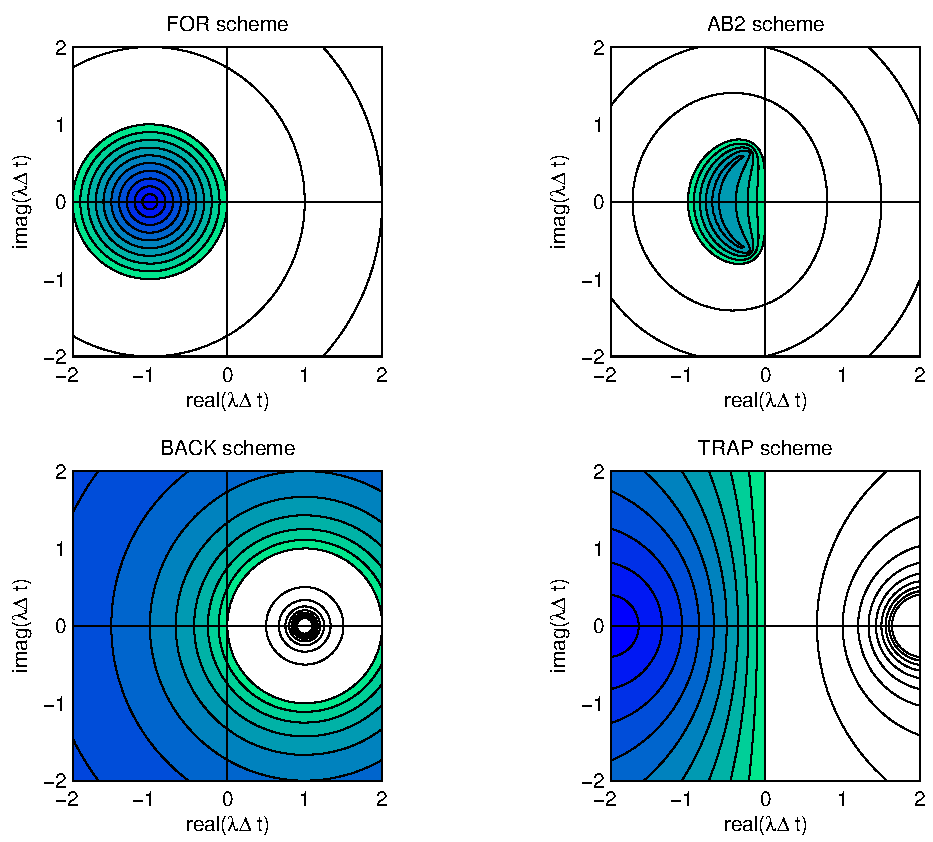
\includegraphics[width=5.5in,clip]{plot4}
\mycaption{\label{fig:plot4}
Absolute stability regions for four one-step schemes.  The stability regions 
are shaded, and the contour interval for the amplification factors
$r=\max_j|r_j|$ are 0.1 for $|r|\le1$ and 1.0 for $|r|>1$.}
\end{center}
\end{figure}

To analyze a semi-implicit method we must use \eqref{eq:test2} as explained
above.  For this problem it turns out that the absolute stability depends on
the products $\alpha=a\dt$ and $\beta=b\dt$.  Specifically, any one-step
semi-implicit method applied to \eqref{eq:test2} yields a solution of the form
\begin{equation}
  \psi^n = [r(\alpha,\beta)]^n \psi^0
\label{eq:abstab:onestep}
\end{equation}
where the complex number $r$ is the amplification factor per time 
step.\footnote{The notation is
inconsistent here:  a superscript on $\psi$ means a time level, whereas $r$ is
raised to the $n$th power.} For example, for the Backward/Forward scheme
\eqref{BACK-FOR} we obtain
\begin{equation}
  r(\alpha,\beta) = \frac{1+\beta}{1-\alpha} .
\label{BAC-FOR:amp}
\end{equation}
More generally, the CLM method \eqref{eq:CLM} applied to \eqref{eq:test2} 
yields a solution of the form
\begin{equation}
  \psi^n = \sum_{j=1}^m d_j[r_j(\alpha,\beta)]^n ,
\label{eq:abstab:mstep}
\end{equation}
where $r_j(\alpha,\beta)$, $j=1,\dots,m$, are the roots of the corresponding
\emph{stability polynomial}
\begin{equation}
  P(z;\alpha,\beta) := \sum_{j=0}^{m} \left(c_j-\alpha a_j - \beta b_j\right)
  z^{m-j} 
\label{eq:cpoly}
\end{equation}
and $d_j$ is a constant (if $r_j$ is a simple root) or a polynomial in $n$ 
of degree less than $q$ (if $r_j$ is a root of multiplicity $q>1$).
For example, for the trapezoidal/leapfrog scheme \eqref{TRAP-LFG} we have
\begin{equation}
  r_{1,2}(\alpha,\beta) = 
    \frac{\beta\pm\sqrt{1 + \beta^2 - \alpha^2}}{1-\alpha} .
\label{TRAP-LFG:amp}
\end{equation}

For each $j=1,\dots,m$, $r_j(\alpha,\beta)$ is the amplification factor for
the corresponding solution mode in~\eqref{eq:abstab:mstep}; the solution is
bounded (for all initial conditions) if and only if these roots satisfy the
root condition \eqref{eq:rootcondition}.  The stability polynomial
\eqref{eq:spoly} and characteristic polynomial \eqref{eq:cpoly} are related by
$P_0(z)=P(z;0,0)$.  Since the roots of a polynomial are continuous functions
of the polynomial coefficients, each root $r_j(\alpha,\beta)$ of
$P(z;\alpha,\beta)$ tends toward a root $r_j$ of $P_0(z)$ as
$\alpha,\beta\to0$ (we will index these roots so that $r_j(0,0)=r_j$,
$j=1,\dots,m$).  Thus, absolute stability implies zero stability but not
conversely.\footnote{More precisely:  if there is a positive time step $\dt_0$
and values of $\alpha$ and $\beta$ such that a given method is absolutely
stable for all $\dt$ in $(0,\dt_0]$ with that $\alpha$ and $\beta$, then the
method is zero-stable.} Also, since $P_0(1)=1$ for a consistent method and we
have set $r_1=1$, we have $r_1(\alpha,\beta)\to1$ as $\alpha,\beta\to0$.  We
identify this root as the \emph{physical mode} and the remaining roots
$r_j(\alpha,\beta)$, $j=2,\dots,m$, as \emph{computational modes}. 

The \emph{region of absolute stability} for a semi-implicit method is the set
of all values $(\alpha,\beta)$ for which $\abs{r_j(\alpha,\beta)}<1$ for
$j=1,\dots,m$.\footnote{Actually, this is the interior of the region; some
points on the boundary may also be included.} Since in general we may regard
$a$ and $b$ in the test equation \eqref{eq:test2} as complex constants, the
stability region is a subset of $\C\times\C$, which (as a vector space over
the reals) is four-dimensional.  Thus, describing that region in general seems
daunting.  Rather, we can consider separately cases where $\alpha$ or $\beta$
is purely real or imaginary and thus reduce the dimension.  Ascher et
al.~\cite{Ascher_Ruuth_Wetton95} considered the case $\alpha$ real (negative)
and $\beta$ pure imaginary, corresponding to the convection-diffusion equation
with the diffusion treated implicitly.  Here we consider the purely
oscillatory case where both $\alpha$ and $\beta$ are pure imaginary,
corresponding to the case of fast and slow waves as in the shallow-water model
above.  In particular, we use $\alpha=i\Omega_f$ and $\beta=i\Omega_s$, with
the real parameters $\Omega_f=\omega_f\dt$ and $\Omega_s=\omega_s\dt$ being
the Courant numbers for the fast components (e.g., gravity waves) and slow
components (e.g., advection), respectively, of the solution.  Thus, we can
evaluate the absolute stability of a scheme (for oscillatory problems) by
plotting the intersection of the stability region with the 
$(\Omega_f,\Omega_s)$-plane.

\pagebreak[2]

An ideal semi-implicit method for oscillatory problems would satisfy the
following criteria:
\begin{enumerate}
\setlength{\itemsep}{2pt} \setlength{\parsep}{0pt}
\setlength{\topsep}{0pt} \setlength{\partopsep}{0pt}
\setlength{\itemsep}{0pt}
\item stable for $\Omega_s=O(1)$ and for all $\Omega_f$,
\item damps the solution for $\abs{\Omega_f}\gg1$,
\item has high-order accuracy.
\end{enumerate}
Condition (1) is the best stability we can hope for, since purely 
explicit schemes have CFL conditions of the form $\Omega_s=O(1)$.
Condition (2) is desirable, since any fast modes with large Courant numbers
will be poorly approximated (although stable), and thus should be removed.
Condition (3) is a major goal of this work, since high accuracy in time may be
beneficial in models with accurate space discretizations, but most
semi-implicit methods used to date are at best second-order accurate.
In the subsections which follow we look for such schemes by considering the
possible schemes in order of increasing number of steps $m$.

\pagebreak[3]
\subsection{One-step semi-implicit schemes}

For a one-step scheme ($m=1$), the requirements \eqref{eq:consistency1} and 
\eqref{eq:consistency2} for consistency reduce the general CLM method 
\eqref{eq:CLM} to
\begin{equation}
  \frac{\psi^{n+1}-\psi^{n}}{\dt} =
    \theta \opA(\psi^{n+1}) + (1-\theta) \opA(\psi^{n}) + \opB(\psi^{n}) ,
\end{equation}
where $\theta$ is the single free parameter.  
From \eqref{eq:terr} the corresponding truncation error is
\begin{equation}
  \tau = \left[\frac12 \opB'(t_n) 
       + \left(\frac12-\theta\right)\opA'(t_n)\right]\dt
       + O\left((\dt)^2\right) .
\end{equation}
Thus, this scheme is first-order accurate, unless $\theta=\frac12$ 
(the trapezoidal implicit scheme) in which case it is second-order accurate in
the implicit terms.  
The corresponding region of absolute stability can be shown to be
\begin{equation}
  \left[\Omega_s + (1-\theta)\Omega_f\right]^2 \le \theta^2\Omega_f^2 .
\end{equation}
Thus, this method is absolutely \emph{unstable} for any $\Omega_s\ne0$.  This
result for forward (Euler) time differencing is of course well-known; here,
it says that there are no one-step semi-implicit methods suitable for use in
oscillatory problems. 

\pagebreak[3]
\subsection{Two-step semi-implicit schemes}

For a two-step scheme ($m=2$), the requirements \eqref{eq:consistency1} 
and \eqref{eq:order} for second-order accuracy reduce the general CLM method 
\eqref{eq:CLM} to
\begin{equation}
\begin{split}
\frac{(\gamma+\tfrac12)\psi^{n+1} - 2\gamma\psi^{n}
        + (\gamma-\tfrac12)\psi^{n-1}}{\dt} 
=& \left(\gamma+\tfrac{c}{2}\right) \opA(\psi^{n+1}) 
    + (1-\gamma-c) \opA(\psi^{n}) + \tfrac{c}{2} \opA(\psi^{n-1})
\nonumber
\\
 & {} + (1+\gamma) \opB(\psi^{n}) - \gamma \opB(\psi^{n-1}) ,
\label{eq:SIm2}
\end{split}
\end{equation}
with two parameters $c$ and $\gamma$ left to specify.
Some special cases include
$(\gamma,c)=(0,1)$ for the trapezoidal/leapfrog scheme
\eqref{TRAP-LFG} and $(\gamma,c)=(\tfrac12,0)$ for a trapezoidal/AB2 
scheme.\footnote{A modified version of this scheme---with an uncentered
first-order implicit scheme---was used by \cite{Simmons_Temperton97}.}
An analysis shows that:
{\setlength{\parskip}{0pt}
\begin{itemize}
\setlength{\itemsep}{2pt} \setlength{\parsep}{0pt}
\setlength{\topsep}{0pt} \setlength{\partopsep}{0pt}
\item Only $\gamma=0$ (leapfrog explicit) gives a nontrivial 
\emph{explicit} stability region, i.e., stability for some $|\Omega_s|>0$.
\item With $\gamma=0$, $c\ge\frac12$ is needed for stability as
$|\Omega_f|\to\infty$.  The stability region is given by
\begin{math}
    \left[\Omega_s + (1-c)\Omega_f\right]^2 \le 1+c^2\Omega_f^2 ,
\end{math}
which includes $|\Omega_s|\le\sqrt{2c-1}/c$. This is maximized by choosing
$c=1$, i.e., the trapezoidal implicit scheme.
\end{itemize}
}
\noindent
Thus, we conclude that of the family \eqref{eq:SIm2} of second-order two-step
semi-implicit schemes, the traditional trapezoidal/leapfrog scheme
\eqref{TRAP-LFG} is best for oscillatory problems.  However, note that it
suffers from two defects:  it has a computational mode which is not
damped, and for large $\Omega_f$ the stability is only marginal, i.e., the
high-frequency modes are not damped.  The absolute stability region for this
scheme is shown in the upper panel of Fig.~\ref{fig:siplot}.

\begin{figure}[bt]
\begin{center}
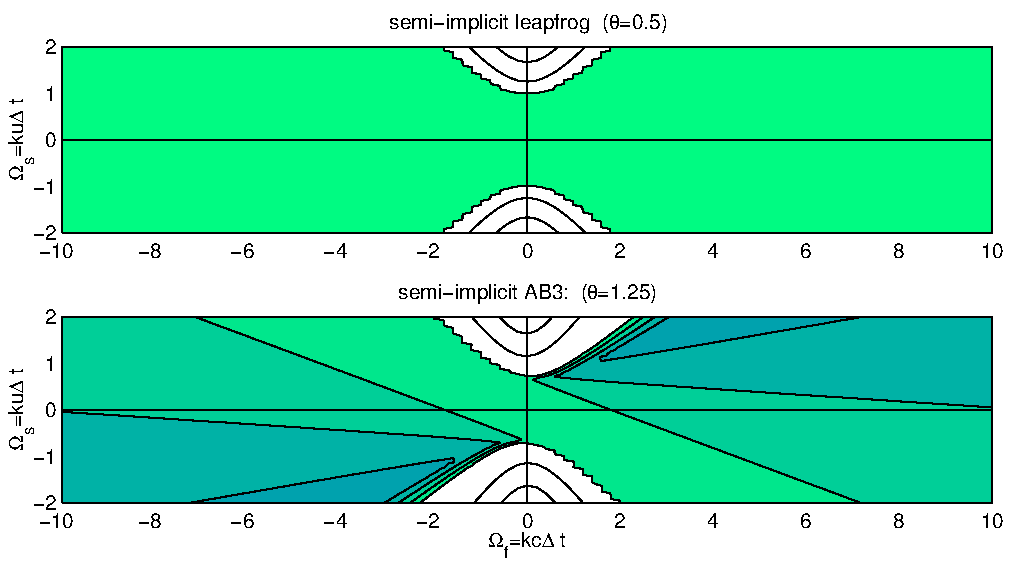
\includegraphics[width=6.5in,clip]{siplot}
\mycaption{\label{fig:siplot}
Amplification factors for the trapezoidal/leapfrog scheme (top panel) 
and the SI2/AB3 scheme (bottom panel) for 
oscillatory problems.  The region of absolute stability is shaded,
and the contour interval for the amplification factor is 0.1 for $|r|\le1$ and 
and 1.0 for $|r|>1$.}
\end{center}
\end{figure}

\pagebreak[3]
\subsection{Three-step semi-implicit schemes (generalized Adams form)}

For a three-step scheme ($m=3$), there are many possibilities.  Here we
consider only schemes with $c_2=c_3=0$, which we refer to as the
\emph{generalized Adams form} (since it generalizes the explicit 
Adams-Bashforth and implicit Adams-Moulton methods).  These schemes have two
distinct advantages:  their computational modes are well-behaved, damping as
$\dt\to0$ (the stability polynomial has a single nonzero root $r_1=1$), 
and they do not require storing past values of $\psi$.  Such schemes take the
form
\begin{alignat}{3}
   \frac{\psi^{n+1}-\psi^{n}}{\dt} = a_0 \opA(\psi^{n+1})
      &+ a_1 \opA(\psi^{n}) &&+ a_2 \opA(\psi^{n-1}) &&+ a_3 \opA(\psi^{n-2})
\nonumber
\\
  &+ b_1 \opB(\psi^{n}) &&+ b_2 \opB(\psi^{n-1}) &&+ b_3 \opB(\psi^{n-2}) .
\label{eq:SI-AB3}
\end{alignat}
Requiring third-order accuracy for the explicit part gives the third-order
Adams-Bashforth method (AB3), i.e.,
\begin{equation}
b_1=\tfrac{23}{12},
\qquad
b_2=-\tfrac{16}{12},
\qquad
b_3= \tfrac{5}{12}.
\label{coeff:AB3}
\end{equation}

If we set $a_3=0$ for simplicity, we can require second-order accuracy for 
the implicit part, yielding the generalized second-order Adams-Moulton 
method (GAM2)
\begin{equation}
a_0 =  \theta,
\qquad
a_1 =  \tfrac32 - 2\theta,
\qquad
a_2 = -\tfrac12 + \theta,
\label{coeff:GAM2}
\end{equation}
where $\theta$ is a free parameter.  Several choices of $\theta$ are of
interest.  The choice $\theta=0$ gives the (explicit) AB2 scheme.
The choice $\theta=\tfrac12$ gives the trapezoidal implicit scheme,
which omits $\psi^{n-1}$.  The choice $\theta=\tfrac{5}{12}$ minimizes the
truncation error, giving the classical third-order Adams-Moulton (AM3) method.
We will refer to the scheme \eqref{eq:SI-AB3} with the coefficients
\eqref{coeff:AB3} and \eqref{coeff:GAM2} as the SI2/AB3 scheme; this scheme
does not appear to have been studied before.  Analysis of this scheme shows:
{\setlength{\parskip}{0pt}
\begin{itemize}
\setlength{\itemsep}{2pt} \setlength{\parsep}{0pt}
\setlength{\topsep}{0pt} \setlength{\partopsep}{0pt}
\item Stability for $|\Omega_f|\to\infty$ (with $|\Omega_s|=0$)
requires $\theta\ge\tfrac12$
\item For $\theta\ge\tfrac{9}{16}$, high frequencies damp with the factor
$\lambda=(\theta-\tfrac12)/\theta$
\item For $\Omega_s\ne0$, the trapezoidal ($\theta=\tfrac12$)
and AM3 ($\theta=\tfrac{5}{12}$) versions are \emph{unstable}
\item For $\theta\approx\tfrac54$, the SI2/AB3 scheme is \emph{stable}
\end{itemize}
}
\noindent
The stability region for the SI2/AB3 scheme with various choices of the free
parameter $\theta$ are shown in Fig.~\ref{fig:si2ab3}.  From these
results it would appear that the optimum stability properties are obtained
when $\theta\approx1.25$.  For comparison with the trapezoidal/leapfrog
scheme, the corresponding absolute stability region is is shown in the lower
panel of Fig.~\ref{fig:siplot}.  

\begin{figure}[hbp]
\begin{center}
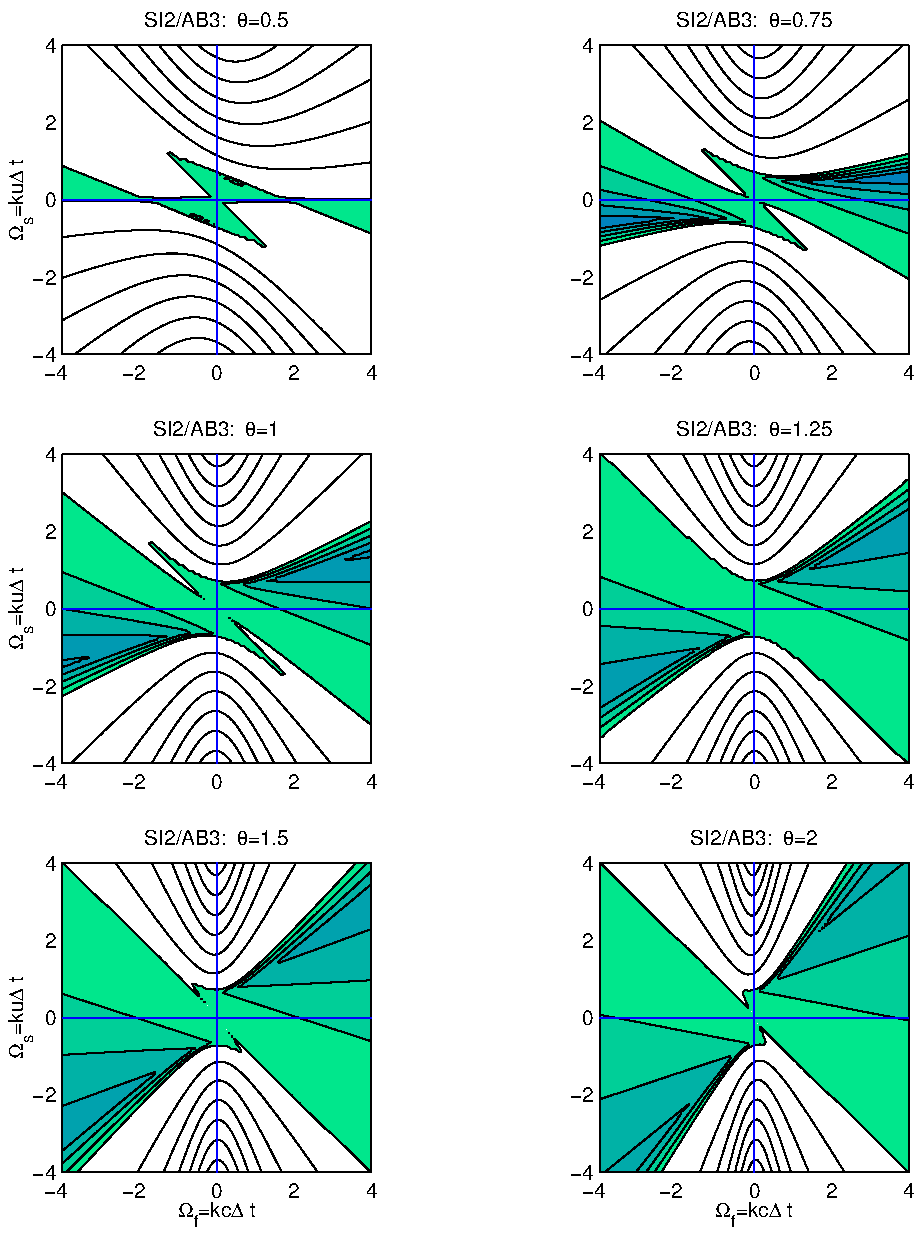
\includegraphics[width=5.5in,clip]{si2ab3}
\mycaption{\label{fig:si2ab3}
Amplification factors for the semi-implicit AB3 scheme for oscillatory 
problems.  
The six panels correspond to the values $\theta=0.5$, 0.75, 1.0, 1.25, 1.5,
and~2 as labeled.  Contours and shading are as in Fig.~\ref{fig:siplot}.}
\end{center}
\end{figure}

If we allow $a_3\ne0$, we can require third-order accuracy, 
yielding the generalized third-order Adams-Moulton method (GAM3)
\begin{equation}
a_0 =  \theta,
\qquad
a_1 =  \tfrac{23}{12} - 3\theta,
\qquad
a_2 = -\tfrac{16}{12} + 3\theta,
\qquad
a_3 =  \tfrac{5}{12} - \theta,
\label{coeff:GAM3}
\end{equation}
where $\theta$ is a free parameter.  Several choices of $\theta$ are of
interest.  The choice $\theta=0$ gives the (explicit) AB3 scheme.  The choice
$\theta=\tfrac{5}{12}$ gives the classical third-order Adams-Moulton (AM3),
which omits $\psi^{n-2}$.  The choice $\theta=\tfrac{3}{8}$ minimizes the
truncation error, giving the classical fourth-order Adams-Moulton (AM4)
method.  We will refer to the scheme \eqref{eq:SI-AB3} with the coefficients
\eqref{coeff:AB3} and \eqref{coeff:GAM3} as the SI3/AB3 scheme.  Preliminary
analysis of this scheme suggests that there is \emph{no} value of $\theta$
which yields adequate absolute stability for oscillatory problems.

\pagebreak[4]
\section{Conclusions\label{sec:conclusions}}
\setcounter{equation}{0}

We have reviewed the formulation semi-implicit time differencing schemes for
the shallow-water equations.  Analysis of the linearized equations identified
the terms which should be treated implicitly.  Splittings based on both the
momentum and vorticity/divergence forms were developed.  Even with a spatially
varying reference depth and the Coriolis terms treated implicitly, in each
formulation the implicit problem to be solved at each time step can be reduced
to a linear elliptic equation (the vorticity/divergence form also requires
solving Poisson problems for the velocity potential and streamfunction).

Analysis of general semi-implicit schemes based on linear multistep methods
shows that combining explicit and implicit schemes which are both convergent 
leads to a convergent method.  The overall order of the scheme is the minimum
of the orders of the implicit and explicit methods used.  However, if there is
little energy in the modes treated implicitly then the overall accuracy may be
that of the explicit method (which may be higher).

A search through part of the vast space of semi-implicit schemes
yielded the following results for purely oscillatory problems of the
type frequently encountered in atmospheric modeling:
{\setlength{\parskip}{0pt}
\begin{itemize}
\setlength{\itemsep}{2pt} \setlength{\parsep}{0pt}
\setlength{\topsep}{0pt} \setlength{\partopsep}{0pt}
\item There are no useful one-step semi-implicit schemes.
\item The best two-step semi-implicit scheme is the widely-used
trapezoidal/leapfrog scheme; however, this includes a non-damped computational
mode, does not damp the poorly-approximated high-frequency modes, and is 
only second-order accurate.
\item The trapezoidal/AB2 scheme used (in modified form) by 
Simmons and Temperton \cite{Simmons_Temperton97} is unstable.
\item The combination of the backward scheme with the third-order
Adams-Bashforth (AB3) scheme is unstable.
\item The combination of the trapezoidal scheme with the third-order
Adams-Bashforth (AB3) scheme is unstable, as concluded by 
Durran \cite{Durran91}
\item There exists a stable three-step scheme which combines the AB3
explicit scheme with a generalized second-order Adams-Moulton implicit scheme.
\end{itemize} 
}
\noindent
It appears that the SI2/AB3 scheme identified here is a promising candidate
for accurate integration of the shallow-water model, and indeed for similar 
atmospheric models which admit fast and slow modes which are both oscillatory.

\pagebreak[4]
\begin{thebibliography}{99}

\bibitem{Ascher_Petzold98}
Ascher, U. M., and L. R. Petzold, 1998:
\textsl{Computer Methods for Ordinary Differential Equations and
Differential-Algebraic Equations.}
Society for Industrial and Applied Mathematics, 314~pp.

\bibitem{Ascher_Ruuth_Wetton95}
Ascher, U. M., S. J. Ruuth, and B. T. R. Wetton, 1995:
Implicit-explicit methods for time-dependent PDE's.
\textsl{SIAM J. Numer. Anal.}, \textbf{32}, 797--823.

%\bibitem{Atkinson89}
%Atkinson, K. E., 1989:
%\textsl{An Introduction to Numerical Analysis}, second edition.
%Wiley, 712~pp.

%\bibitem{Cooper_Sayfy80}
%Cooper, G. J., and A. Sayfy, 1980:
%Additive methods for the numerical solution of ordinary differential equations.
%\textsl{Math. Comput.}, \textbf{35}, 1980, 1159--1172.

%\bibitem{Cooper_Sayfy83}
%Cooper, G. J., and A. Sayfy, 1983:
%Additive Runge-Kutta methods for stiff ordinary differential equations.
%\textsl{Math. Comput.}, \textbf{40}, 1983, 207--218.

\bibitem{Cote_Beland_Staniforth83}
C\^{o}t\'{e}, J., M. B\'{e}land, and A. Staniforth, 1983:
Stability of vertical discretization schemes for semi-implicit primitive
equation models:  Theory and application.
\textsl{Mon.\ Wea.\ Rev.}, \textbf{111}, 1189--1207.

\bibitem{Durran91}
Durran, D. R., 1991:
The third-order Adams-Bashforth method:  An attractive alternative to leapfrog
time differencing.
\textsl{Mon.\ Wea.\ Rev.}, \textbf{119}, 702--720.

\bibitem{Fulton93}
Fulton, S. R., 1993:
A semi-implicit spectral method for the anelastic equations.
\textsl{J.~Comp.\ Phys.}, \textbf{106}, 299--305.

%\bibitem{Fulton02}
%Fulton, S. R., 2002:
%Semi-implicit time differencing.
%Technical Report No.~2002-01,
%Department of Mathematics and Computer Science,
%Clarkson University, Potsdam, NY 13699--5815

\bibitem{Fulton_Schubert87b}
Fulton, S. R., and W. H. Schubert, 1987:
Chebyshev spectral methods for limited-area models.
Part~II:  Shallow water model.
\textsl{Mon.\ Wea.\ Rev.}, \textbf{115}, 1954--1965.

\bibitem{Heikes_Randall95a}
Heikes, R., and D. A. Randall, 1995:
Numerical integration of the shallow-water equations on a twisted icosahedral
grid.  Part~I:  Basic design and results of tests.
\textsl{Mon.\ Wea.\ Rev.}, \textbf{123}, 1862--1880.

\bibitem{Lambert91}
Lambert, J. D., 1991: 
\textsl{Numerical Methods for Ordinary Differential Systems.}
Wiley, 293~pp.

\bibitem{Kang94}
Kang, Y., 1994:
Analysis and Applications of Combined Numerical Methods 
for Systems of Differential Equations.
Ph.D. Dissertation, Department of Mathematics and Computer Science,
Clarkson University, 157~pp.

\bibitem{Kwizak_Robert71}
Kwizak, M. and A. J. Robert, 1971:
A semi-implicit scheme for gridpoint atmospheric models of the primitive
equations.
\textsl{Mon.\ Wea.\ Rev.}, \textbf{99}, 32--36.

%\bibitem{Robert_Henderson_Turnbull72}
%Robert, A. J., J. Henderson, and C. Turnbull, 1972:
%An implicit time integration scheme for baroclinic modes of the atmosphere. 
%\textsl{Mon.\ Wea.\ Rev.}, \textbf{100}, 329--335.

\bibitem{Sadun01}
Sadun, L., 2001:
\textsl{Applied Linear Algebra}.
Prentice-Hall, 349~pp.

\bibitem{Simmons_Hoskins_Burridge78}
Simmons, A. J., B. J. Hoskins, and D. M. Burridge, 1978:
Stability of the semi-implicit method of time integration.
\textsl{Mon.\ Wea.\ Rev.}, \textbf{106}, 405--412.

\bibitem{Simmons_Temperton97}
Simmons, A. J., and C. Temperton, 1997:
Stability of a two-time-level semi-implicit integration scheme for gravity
wave motion.
\textsl{Mon.\ Wea.\ Rev.}, \textbf{125}, 600--615.

\bibitem{Staniforth_Daley79}
Staniforth, A., and R. W. Daley, 1979:
A baroclinic finite-element model for regional forecasting with the primitive
equations.
\textsl{Mon.\ Wea.\ Rev.}, \textbf{107}, 107--121.

\bibitem{Stoer_Bulirsch92}
Stoer, J., and R. Bulirsch, 1992:
\textsl{Introduction to Numerical Analysis}, second edition.
Springer, 660~pp.

\end{thebibliography}

%\pagebreak[3]
%\appendix
%\section*{\label{sec:sitpack}Appendix:
%Software for Semi-Implicit Schemes}

\end{document}

One question remains:  should we treat the Coriolis terms implicitly or
explicitly?  On one hand, their time scale is much slower, so there is no
apparent need to treat them implicitly.  On the other hand, since they are
linear, including them in the problem to be solved implicitly might not be too
difficult, and perhaps may have some advantage (e.g., smaller truncation
error).  In addition, the above analysis suggests another reason to treat them
implicitly as follows.  Treating $C$ implicitly means splitting the operator
$L$ in \eqref{SW:matrix} into $A+C$ and  $B$.  Since $B=-i\omegabar I$, it
commutes with $A+C$, so these operators are simultaneously orthogonally
diagonalizable \cite{Sadun01}.  This means that the absolute stability
analysis of section~\ref{sec:abstab} applies directly (at least to this linear
problem), giving some confidence that methods which the analysis identifies as
good will in fact work properly.  On the other hand, treating $C$ explicitly
means splitting the operator $L$ in (\ref{SW:matrix}) into $A$ and  $B+C$.
Since these two operators do not commute, they are not simultaneously
orthogonally diagonalizable, and the applicability of the absolute stability
analysis is unclear.  In this sense, therefore, it would be natural to treat
the Coriolis terms implicitly.  However, since the contribution from these
terms is relatively small, there may be little difference in practice, and
treating these terms explicitly may be simpler.
